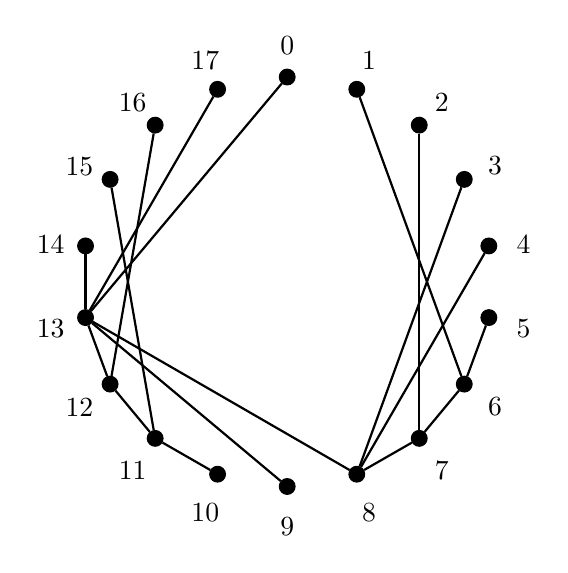
\begin{tikzpicture}
	\tikzset{enclosed/.style={draw, circle, inner sep=0pt, minimum size=0.2cm, fill=black}}

	\node[enclosed, label={above, xshift=0cm, yshift=0.052cm:0}] at (3.38, 5.2)(0){};
	\node[enclosed, label={above, xshift=0.156cm, yshift=0.026cm:1}] at (4.264, 5.044)(1){};
	\node[enclosed, label={above, xshift=0.286cm, yshift=-0.052cm:2}] at (5.057, 4.589)(2){};
	\node[enclosed, label={above, xshift=0.39cm, yshift=-0.169cm:3}] at (5.629, 3.9)(3){};
	\node[enclosed, label={above, xshift=0.442cm, yshift=-0.325cm:4}] at (5.941, 3.055)(4){};
	\node[enclosed, label={above, xshift=0.442cm, yshift=-0.481cm:5}] at (5.941, 2.145)(5){};
	\node[enclosed, label={above, xshift=0.39cm, yshift=-0.624cm:6}] at (5.629, 1.3)(6){};
	\node[enclosed, label={above, xshift=0.286cm, yshift=-0.754cm:7}] at (5.057, 0.611)(7){};
	\node[enclosed, label={above, xshift=0.156cm, yshift=-0.832cm:8}] at (4.264, 0.156)(8){};
	\node[enclosed, label={above, xshift=0cm, yshift=-0.858cm:9}] at (3.38, 0)(9){};
	\node[enclosed, label={above, xshift=-0.156cm, yshift=-0.832cm:10}] at (2.496, 0.156)(10){};
	\node[enclosed, label={above, xshift=-0.286cm, yshift=-0.754cm:11}] at (1.703, 0.611)(11){};
	\node[enclosed, label={above, xshift=-0.39cm, yshift=-0.637cm:12}] at (1.131, 1.3)(12){};
	\node[enclosed, label={above, xshift=-0.442cm, yshift=-0.481cm:13}] at (0.819, 2.145)(13){};
	\node[enclosed, label={above, xshift=-0.442cm, yshift=-0.325cm:14}] at (0.819, 3.055)(14){};
	\node[enclosed, label={above, xshift=-0.39cm, yshift=-0.182cm:15}] at (1.131, 3.9)(15){};
	\node[enclosed, label={above, xshift=-0.286cm, yshift=-0.052cm:16}] at (1.703, 4.589)(16){};
	\node[enclosed, label={above, xshift=-0.156cm, yshift=0.026cm:17}] at (2.496, 5.044)(17){};
	\draw [thick] (0)--(13);
	\draw [thick] (6)--(1);
	\draw [thick] (6)--(5);
	\draw [thick] (7)--(2);
	\draw [thick] (7)--(6);
	\draw [thick] (8)--(3);
	\draw [thick] (8)--(4);
	\draw [thick] (8)--(7);
	\draw [thick] (11)--(10);
	\draw [thick] (11)--(15);
	\draw [thick] (12)--(11);
	\draw [thick] (12)--(16);
	\draw [thick] (13)--(8);
	\draw [thick] (13)--(9);
	\draw [thick] (13)--(12);
	\draw [thick] (13)--(14);
	\draw [thick] (13)--(17);
\end{tikzpicture}

